\documentclass[tikz,border=10pt]{standalone}
\usepackage{tikz}
\usetikzlibrary{shapes, arrows.meta, positioning, fit, backgrounds, decorations.pathreplacing, calc}

\begin{document}

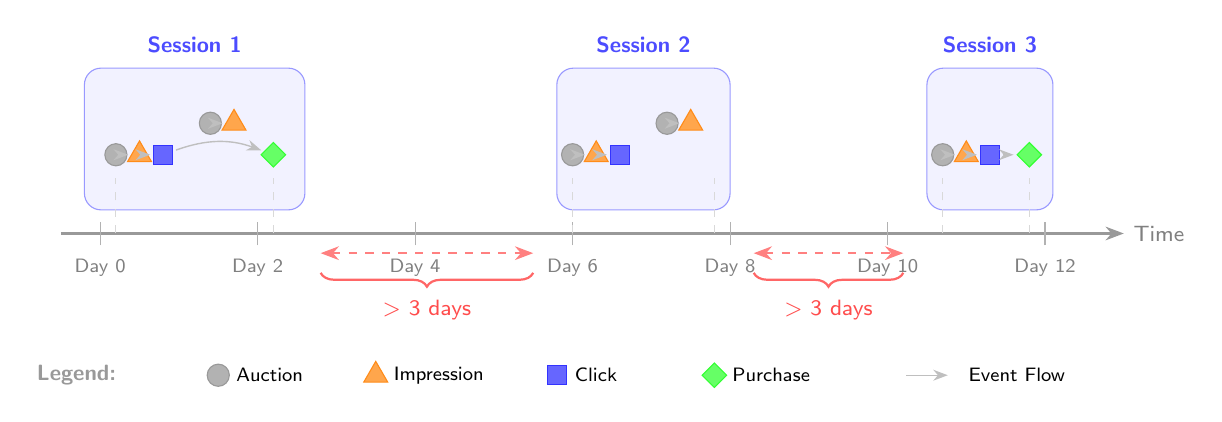
\begin{tikzpicture}[
    >=Stealth,
    % Event marker styles
    auction/.style={circle, fill=gray!60, draw=gray!80, minimum size=8pt, inner sep=0pt},
    impression/.style={regular polygon, regular polygon sides=3, fill=orange!70, draw=orange!90, minimum size=10pt, inner sep=0pt},
    click/.style={rectangle, fill=blue!60, draw=blue!80, minimum size=7pt, inner sep=0pt},
    purchase/.style={diamond, fill=green!60, draw=green!80, minimum size=9pt, inner sep=0pt},
    % Session box style
    sessionbox/.style={rectangle, rounded corners=6pt, draw=blue!40, fill=blue!5, minimum height=1.8cm},
    % Flow connector style
    flow/.style={->, gray!50, line width=0.5pt, shorten >=1pt, shorten <=1pt},
    % Gap annotation style
    gapbrace/.style={decorate, decoration={brace, amplitude=5pt, mirror}, red!60, thick},
    gaplabel/.style={font=\sffamily\footnotesize, red!70},
    % Day label style
    daylabel/.style={font=\sffamily\scriptsize, gray}
]

    % === TIMELINE ===
    \draw[->, thick, gray!80] (-0.5,0) -- (13,0);
    \node[anchor=west, font=\sffamily\footnotesize, gray] at (13,0) {Time};

    % Day tick marks
    \foreach \x/\d in {0/0, 2/2, 4/4, 6/6, 8/8, 10/10, 12/12} {
        \draw[gray!60] (\x,-0.15) -- (\x,0.15);
        \node[daylabel, below] at (\x,-0.2) {Day \d};
    }

    % === SESSION 1 (Days 0-2) ===
    \node[sessionbox, minimum width=2.8cm] (s1box) at (1.2,1.2) {};
    \node[font=\sffamily\footnotesize\bfseries, blue!70, above=2pt of s1box] {Session 1};

    % Events in Session 1
    \node[auction] (a1) at (0.2,1.0) {};
    \node[impression] (i1) at (0.5,1.0) {};
    \node[click] (c1) at (0.8,1.0) {};

    \node[auction] (a2) at (1.4,1.4) {};
    \node[impression] (i2) at (1.7,1.4) {};

    \node[purchase] (p1) at (2.2,1.0) {};

    % Flow connectors Session 1
    \draw[flow] (a1) -- (i1);
    \draw[flow] (i1) -- (c1);
    \draw[flow] (a2) -- (i2);
    \draw[flow, bend left=20] (c1) to (p1);

    % Vertical lines to timeline
    \draw[gray!30, dashed] (0.2,0) -- (0.2,0.7);
    \draw[gray!30, dashed] (2.2,0) -- (2.2,0.7);

    % === SESSION 2 (Days 6-7.5) ===
    \node[sessionbox, minimum width=2.2cm] (s2box) at (6.9,1.2) {};
    \node[font=\sffamily\footnotesize\bfseries, blue!70, above=2pt of s2box] {Session 2};

    % Events in Session 2
    \node[auction] (a3) at (6.0,1.0) {};
    \node[impression] (i3) at (6.3,1.0) {};
    \node[click] (c2) at (6.6,1.0) {};

    \node[auction] (a4) at (7.2,1.4) {};
    \node[impression] (i4) at (7.5,1.4) {};

    % Flow connectors Session 2
    \draw[flow] (a3) -- (i3);
    \draw[flow] (i3) -- (c2);
    \draw[flow] (a4) -- (i4);

    % Vertical lines to timeline
    \draw[gray!30, dashed] (6.0,0) -- (6.0,0.7);
    \draw[gray!30, dashed] (7.8,0) -- (7.8,0.7);

    % === SESSION 3 (Days 11-12) ===
    \node[sessionbox, minimum width=1.6cm] (s3box) at (11.3,1.2) {};
    \node[font=\sffamily\footnotesize\bfseries, blue!70, above=2pt of s3box] {Session 3};

    % Events in Session 3
    \node[auction] (a5) at (10.7,1.0) {};
    \node[impression] (i5) at (11.0,1.0) {};
    \node[click] (c3) at (11.3,1.0) {};
    \node[purchase] (p2) at (11.8,1.0) {};

    % Flow connectors Session 3
    \draw[flow] (a5) -- (i5);
    \draw[flow] (i5) -- (c3);
    \draw[flow] (c3) -- (p2);

    % Vertical lines to timeline
    \draw[gray!30, dashed] (10.7,0) -- (10.7,0.7);
    \draw[gray!30, dashed] (11.8,0) -- (11.8,0.7);

    % === GAP ANNOTATIONS ===
    % Gap 1: between Session 1 and Session 2
    \draw[gapbrace] (2.8,-0.5) -- node[gaplabel, below=6pt] {$>$ 3 days} (5.5,-0.5);
    \draw[<->, red!50, dashed, thick] (2.8,-0.25) -- (5.5,-0.25);

    % Gap 2: between Session 2 and Session 3
    \draw[gapbrace] (8.3,-0.5) -- node[gaplabel, below=6pt] {$>$ 3 days} (10.2,-0.5);
    \draw[<->, red!50, dashed, thick] (8.3,-0.25) -- (10.2,-0.25);

    % === LEGEND ===
    \begin{scope}[shift={(0,-1.8)}]
        \node[font=\sffamily\footnotesize\bfseries, gray!80] at (-0.3,0) {Legend:};

        \node[auction] at (1.5,0) {};
        \node[font=\sffamily\scriptsize, right=3pt] at (1.5,0) {Auction};

        \node[impression] at (3.5,0) {};
        \node[font=\sffamily\scriptsize, right=3pt] at (3.5,0) {Impression};

        \node[click] at (5.8,0) {};
        \node[font=\sffamily\scriptsize, right=3pt] at (5.8,0) {Click};

        \node[purchase] at (7.8,0) {};
        \node[font=\sffamily\scriptsize, right=3pt] at (7.8,0) {Purchase};

        \draw[flow] (10.2,0) -- (10.8,0);
        \node[font=\sffamily\scriptsize, right=3pt] at (10.8,0) {Event Flow};
    \end{scope}

\end{tikzpicture}

\end{document}
